%!TEX program = xelatex
\documentclass[12pt,a4paper]{exam-zh}

\usepackage{amsmath,array,graphicx,booktabs,multirow}
\usepackage{enumitem}
\usepackage{fancyhdr}
\usepackage{tikz}
\usepackage{tabularx}
\usepackage{setspace}
\setCJKmainfont{Noto Serif CJK SC}
\geometry{margin=2.2cm,top=2.0cm,bottom=2.2cm}
\pagestyle{fancy}
\fancyhf{}
\cfoot{-\thepage{}-}
\renewcommand{\headrulewidth}{0pt}
\renewcommand{\footrulewidth}{0pt}
\setlength{\parindent}{0pt}
\setlength{\parskip}{0.2em}
\setlength{\headheight}{14pt}
\linespread{1.12}
\usepackage{setspace}
\usepackage{eso-pic}
\usetikzlibrary{calc}

%region exam setup

\examsetup{
    page = {
    size = a4paper,           % 设定纸张大小 [4]
    foot-content = { - ; - }  % 页脚显示为 -1-, -2- 格式 [3]
  },
    choices = {
    label-pos = top-left,
    column-sep = 1em,
    label-pos = auto,
    label-sep = 0.5em,
    max-columns = 4
    },
  question = {
    top-sep    = 1em, % 调整题目上方的垂直距离（默认值为 .5em plus .5em minus .2em）
    bottom-sep = 1em  % 调整题目下方的垂直距离（默认值为 .5em plus .5em minus .2em）
  },
    paren = {
    show-paren = false  % 设置为 false 则不显示括号 [3, 4]
  },
    choices = {
    label = \textbf{\Alph*}
  }, 
    solution = {
    show-solution = show-move, % 答案自动移动到卷末
    label-content = {参考答案},  % 答案区的标题文字
    show-qed = true            % 在解答末尾显示结束符号 ◻ 
  }
}

%endregion


%region 卷面变量设置
    % ==========================
    % ==========================
% 卷面变量设置（只需改这里）
% ==========================
\newcommand{\papercode}{SC 07}
\newcommand{\examtitle}{2026年金宝培元独立中学八月考}
\newcommand{\examlevel}{高中组}
\newcommand{\examsubject}{高级数学(II)}
\newcommand{\sidebartext}{高级数学(II)}
\newcommand{\papername}{试卷一}
\newcommand{\papertype}{选择题}
\newcommand{\examdate}{2026年8月6日}
\newcommand{\examtime}{10.15 a.m.－11.00 a.m.}
\newcommand{\examduration}{45分钟}
\newcommand{\questionpages}{4面}
\newcommand{\paperonepercentage}{40\%}
\newcommand{\papertwopercentage}{60\%}
\newcommand{\setterteacher}{蔡杰庆师}
\newcommand{\reviewteacher}{王萌师}
\newcommand{\auditteacher}{雷泳健师}
    \newcommand{\optrow}[4]{%
    \begin{tabular*}{\linewidth}{@{\extracolsep{\fill}}llll}
    A~#1 & B~#2 & C~#3 & D~#4
    \end{tabular*}%
    }
    \newcommand{\qitem}[5]{\item #1\par\optrow{#2}{#3}{#4}{#5}}
%endregion
    \begin{document}


%region 封面
    \AddToShipoutPictureFG*{%
    \put(31,104){\color{black}\rule{16pt}{66pt}}%
    \put(37,112){\makebox(0,0)[lb]{\rotatebox{90}{\color{white}\bfseries\footnotesize \sidebartext}}}%
    \put(24,18){\makebox(0,0)[lb]{\small 版权所有}}%
    \put(520,18){\makebox(0,0)[lb]{\bfseries\small 【机密】}}%
    }

    \thispagestyle{fancy}

    \begin{minipage}[t]{0.22\linewidth}
    \vspace{0pt}
    \end{minipage}
    \hfill
    \begin{minipage}[t]{0.56\linewidth}
    \centering
    {\zihao{3}\bfseries \examtitle\par}
    \vspace{2.3em}
    {\zihao{3}\bfseries \examlevel\par}
    \vspace{0.3em}
    {\zihao{2}\bfseries \examsubject\par}
    \vspace{0.2em}
    {\large (\papercode)\par}
    \end{minipage}
    \hfill
    \begin{minipage}[t]{0.18\linewidth}
    \vspace{0pt}
    \end{minipage}

    \vspace{3.0em}

    \begin{center}
    \begin{tabular}{c}
        \papername\hspace{2em}\papertype\\[-0.1em]
        \midrule
        日期:\examdate\\[-0.1em]
        时间:\examtime\\[-0.1em]
        (\examduration)\\
        \midrule
    \end{tabular}
    \end{center}

    \vspace{2.0em}

    {\zihao{4}\bfseries \underline{考生须知}\par}
    \vspace{0.8em}

    \begin{enumerate}[label=\arabic*、,leftmargin=2em,itemsep=0.65em]
    \item 本科试卷共分两份：\\
    试卷一：选择题（\paperonepercentage）；\\
    试卷二：作答题（\papertwopercentage）。

    \item 考生须于第一阶段规定的60分钟内完成试卷一。第二阶段规定的2小时内作答试卷二。

    \item 试卷一选择题20题全答。选出正确的答案，然后用\textbf{5B铅笔将“O”答案纸}（电脑卡）上相应的字母所在的小方格涂黑。

    \item 可使用电子计算机进行演算。

    \item 试卷一选择题共印\questionpages。
    \end{enumerate}

    \vspace{2.0em}

    \begin{center}
    {\setlength{\fboxrule}{1.2pt}\fbox{\rule{0pt}{1.1em}\hspace{1.2em}{\zihao{4}\bfseries 未经正式宣布\quad 不得翻看内页}\hspace{1.2em}}}
    \end{center}

    \vfill

    \begin{tabular*}{\linewidth}{@{\extracolsep{\fill}}ll}
    考生姓名：\underline{\hspace{4.2cm}} & 考生编号：\underline{\hspace{4.0cm}}
    \end{tabular*}

%endregion

\newpage



%region 范围：复数 | 考点：复数乘 i 对辐角的影响 | 难度：困难
\begin{question}
    已知 $\alpha$ 为复数 $z=x+yi$ 的辐角，$\beta$ 为复数 $-y+xi$ 的辐角且$0 < \alpha < \beta < 2\pi$，求 $\alpha-\beta$。 \paren[2]
    \begin{choices}
        \item $\dfrac{\pi}{2}$
        \item $-\dfrac{\pi}{2}$
        \item $\pi$
        \item $-\pi$
    \end{choices}
\end{question}

\begin{solution}
    已知 $\alpha$ 为复数 $z=x+yi$ 的辐角，$\beta$ 为复数 $-y+xi$ 的辐角，求 $\alpha-\beta$。 \\
    注意到 $-y+xi=i(x+yi)=iz$，乘以 $i$ 使辐角增加 $\dfrac{\pi}{2}$。 \\
    \begin{align*}
        -y+xi &= i(x+yi) \\
        &= iz
    \end{align*}
    \[
        \beta = \arg(iz) = \alpha+\frac{\pi}{2}
    \]
    \[
        \alpha-\beta = -\frac{\pi}{2}
    \]
    故选 B。
\end{solution}
%endregion



%region 范围：复数 | 考点：i 的周期性（i^n 循环节） | 难度：中等
\begin{question}
    $i^3+i^7+i^{11}+i^{15}+\cdots+i^{399}$ 的值为？ \paren[2]
    \begin{choices}
        \item $0$
        \item $i$
        \item $-100i$
        \item $-99i$
    \end{choices}
\end{question}

\begin{solution}
    $i^3+i^7+i^{11}+i^{15}+\cdots+i^{399}$ 的值为？ \\
    各项指数为 $4k+3$，而 $i^{4k+3}=i^{4k}\cdot i^3=-i$，先求项数再乘 $-i$。 \\
    \begin{align*}
        \text{项数} &= \frac{399-3}{4}+1 \\
        &= 100
    \end{align*}
    \[
        i^3+i^7+\cdots+i^{399} = 100\times(-i) = -100i
    \]
    故选 C。
\end{solution}
%endregion

%region 范围：复数 | 考点：复数的模与象限判断 | 难度：基础
\begin{question}
    已知复数 $z=-\sqrt{3}+bi$（$b\in\mathbb{R}$）在复平面上对应的点位于第三象限，且 $|z|=2$，求 $b$。 \paren[2]
    \begin{choices}
        \item $1$
        \item $-1$
        \item $\pm1$
        \item $-\sqrt{3}$
    \end{choices}
\end{question}

\begin{solution}
    已知复数 $z=-\sqrt{3}+bi$ 在复平面上对应的点位于第三象限，且 $|z|=2$，求 $b$。 \\
    先由模长求出 $b$ 的两个可能值，再用第三象限的条件（虚部为负）取舍。 \\
    \begin{align*}
        \sqrt{(-\sqrt3)^2+b^2} &= 2 \\
        3+b^2 &= 4 \\
        b^2 &= 1 \\
        b &= \pm1
    \end{align*}
    \[
        \text{第三象限} \implies b<0 \implies b=-1
    \]
    故选 B。
\end{solution}
%endregion

%region 范围：复数 | 考点：复数方程求解 | 难度：中等
\begin{question}
    已知复数 $z=-\dfrac{1}{2}+mi$（$m\in\mathbb{R}$），且 $z^4=z$，求 $m$。 \paren[2]
    \begin{choices}
        \item $\dfrac{\sqrt3}{2}$
        \item $-\dfrac{\sqrt3}{2}$
        \item $\pm\dfrac{\sqrt3}{2}$
        \item $\pm\sqrt3$
    \end{choices}
\end{question}

\begin{solution}
    已知复数 $z=-\dfrac{1}{2}+mi$，且 $z^4=z$，求 $m$。 \\
    $z$ 的实部非 $0$ 故 $z\neq0$，两边同除 $z$ 得 $z^3=1$，展开实部并令其为 $1$ 即可解出 $m$。 \\
    \begin{align*}
        \left(-\frac{1}{2}+mi\right)^3 &= 1 \\
        -\frac{1}{8}+\frac{3}{2}m^2 &= 1 \\
        m^2 &= \frac{3}{4} \\
        m &= \pm\frac{\sqrt{3}}{2}
    \end{align*}
    故选 C。
\end{solution}
%endregion

%region 范围：复数 | 考点：复数的三角形式 | 难度：中等
\begin{question}
    将复数 $\dfrac{\sqrt{2}}{1-i}$ 化为三角函数式。 \paren[A]
    \begin{choices}[columns=2, linesep=0.5em]
        \item $\cos\dfrac{\pi}{4}+i\sin\dfrac{\pi}{4}$
        \item $2\left(\cos\dfrac{\pi}{4}+i\sin\dfrac{\pi}{4}\right)$
        \item $\cos\dfrac{\pi}{4}-i\sin\dfrac{\pi}{4}$
        \item $\cos\dfrac{3\pi}{4}+i\sin\dfrac{3\pi}{4}$
    \end{choices}
\end{question}

\begin{solution}
    将复数 $\dfrac{\sqrt{2}}{1-i}$ 化为三角形式。 \\
    分子分母同乘 $1-i$ 的共轭复数，化为 $a+bi$ 后求模与辐角。 \\
    \begin{align*}
        \frac{\sqrt{2}}{1-i} &= \frac{\sqrt{2}(1+i)}{(1-i)(1+i)} \\
        &= \frac{\sqrt{2}(1+i)}{2} \\
        &= \frac{\sqrt{2}}{2}+\frac{\sqrt{2}}{2}i
    \end{align*}
    \begin{align*}
        r &= \sqrt{\left(\frac{\sqrt{2}}{2}\right)^2+\left(\frac{\sqrt{2}}{2}\right)^2} = 1 \\
        \theta &= \frac{\pi}{4}
    \end{align*}
    \[
        \frac{\sqrt{2}}{1-i} = \cos\frac{\pi}{4}+i\sin\frac{\pi}{4}
    \]
    故选 A。
\end{solution}
%endregion

%region 范围：圆锥曲线 | 考点：由一般式判断二次曲线的类型 | 难度：基础
\begin{question}
    方程式 $4x^2-9y^2+8x-18y-12=0$ 的图像是？ \paren[2]
    \begin{choices}
        \item 圆
        \item 抛物线
        \item 椭圆
        \item 双曲线
    \end{choices}
\end{question}

\begin{solution}
    方程式 $4x^2-9y^2+8x-18y-12=0$ 的图像是？ \\
    配方化为标准式，看 $x^2,y^2$ 系数的符号关系判断曲线类型。 \\
    \begin{align*}
        4(x^2+2x)-9(y^2+2y)-12 &= 0 \\
        4\left[(x+1)^2-1\right]-9\left[(y+1)^2-1\right]-12 &= 0 \\
        4(x+1)^2-9(y+1)^2 &= 7
    \end{align*}
    \[
        x^2,y^2 \text{ 系数异号，右边} \neq 0 \implies \text{双曲线}
    \]
    故选 D。
\end{solution}
%endregion

%region 范围：圆锥曲线 | 考点：配方化椭圆标准式求离心率 | 难度：中等
\begin{question}
    求曲线 $x^2+4y^2+8x-16y-17=0$ 的离心率。 \paren[2]
    \begin{choices}
        \item $\dfrac{1}{2}$
        \item $\dfrac{\sqrt3}{2}$
        \item $\sqrt3$
        \item $\dfrac{2}{7}$
    \end{choices}
\end{question}

\begin{solution}
    求曲线 $x^2+4y^2+8x-16y-17=0$ 的离心率。 \\
    先配方化为椭圆标准式，再由 $a,b$ 求 $c$，代入 $e=\dfrac{c}{a}$。 \\
    \begin{align*}
        (x+4)^2-16+4\left[(y-2)^2-4\right]-17 &= 0 \\
        (x+4)^2+4(y-2)^2 &= 49 \\
        \frac{(x+4)^2}{49}+\frac{(y-2)^2}{49/4} &= 1
    \end{align*}
    \begin{align*}
        a^2=49,\ b^2 &= \frac{49}{4} \\
        c^2 = a^2-b^2 &= \frac{147}{4} \\
        e=\frac{c}{a} &= \frac{\sqrt3}{2}
    \end{align*}
    故选 B。
\end{solution}
%endregion



%region 范围：圆锥曲线 | 考点：双曲线渐近线与直线围成的三角形面积 | 难度：中等
\begin{question}
    已知双曲线 $\dfrac{x^2}{9}-\dfrac{y^2}{4}=1$，求其渐近线与直线 $x=3$ 所围成的三角形的面积。 \paren[2]
    \begin{choices}
        \item $4$
        \item $6$
        \item $9$
        \item $12$
    \end{choices}
\end{question}

\begin{solution}
    已知双曲线 $\dfrac{x^2}{9}-\dfrac{y^2}{4}=1$，求其渐近线与直线 $x=3$ 所围成的三角形的面积。 \\
    渐近线为 $y=\pm\dfrac{b}{a}x$，与 $x=3$ 的交点即三角形另两个顶点，底为交点间的距离，高为原点到 $x=3$ 的距离。 \\
    \begin{align*}
        y &= \pm\frac{2}{3}x \\
        x=3 &\implies y=\pm2
    \end{align*}
    \begin{align*}
        \text{底} &= 2-(-2)=4 \\
        \text{高} &= 3 \\
        S &= \frac{1}{2}\times4\times3=6
    \end{align*}
    故选 B。
\end{solution}
%endregion

%region 范围：圆锥曲线 | 考点：直角双曲线（等轴双曲线）方程的建立 | 难度：中等
\begin{question}
    求以 $(0,-2)$、$(0,6)$ 为焦点的直角双曲线方程。 \paren[2]
    \begin{choices}
        \item $\dfrac{(y-2)^2}{8}-\dfrac{x^2}{8}=1$
        \item $\dfrac{y^2}{8}-\dfrac{x^2}{8}=1$
        \item $\dfrac{(y-2)^2}{16}-\dfrac{x^2}{16}=1$
        \item $\dfrac{x^2}{8}-\dfrac{(y-2)^2}{8}=1$
    \end{choices}
\end{question}

\begin{solution}
    求以 $(0,-2)$、$(0,6)$ 为焦点的直角双曲线方程。 \\
    中心为两焦点中点，$c$ 为中心到焦点的距离；直角双曲线满足 $a=b$，故 $c^2=2a^2$。 \\
    \begin{align*}
        \text{中心} &= (0,2) \\
        c &= 4
    \end{align*}
    \begin{align*}
        c^2 &= 2a^2 \\
        16 &= 2a^2 \\
        a^2=b^2 &= 8
    \end{align*}
    \[
        \frac{(y-2)^2}{8}-\frac{x^2}{8}=1
    \]
    故选 A。
\end{solution}
%endregion

%region 范围：圆锥曲线 | 考点：双曲线的图像识别 | 难度：基础
\begin{question}
    下列哪个图像表示 $x^2-y^2=1$？ \paren[2]
    \begin{choices}[columns=2, linesep=0.5em]
        \item 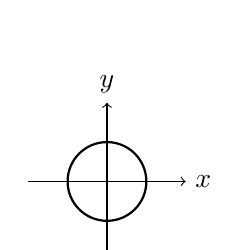
\begin{tikzpicture}[scale=0.5]
            \draw[->] (-2,0)--(2,0) node[right]{$x$};
            \draw[->] (0,-2)--(0,2) node[above]{$y$};
            \draw[thick] (0,0) circle (1);
        \end{tikzpicture}
        \item 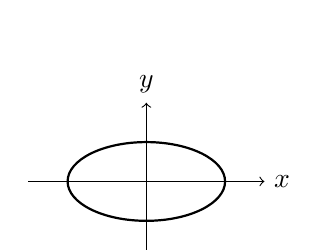
\begin{tikzpicture}[scale=0.5]
            \draw[->] (-3,0)--(3,0) node[right]{$x$};
            \draw[->] (0,-2)--(0,2) node[above]{$y$};
            \draw[thick] (0,0) ellipse (2 and 1);
        \end{tikzpicture}
        \item 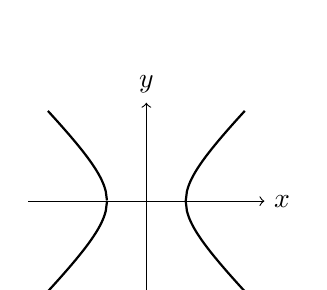
\begin{tikzpicture}[scale=0.5]
            \draw[->] (-3,0)--(3,0) node[right]{$x$};
            \draw[->] (0,-2.5)--(0,2.5) node[above]{$y$};
            \draw[thick,domain=1:2.5,samples=50] plot (\x,{sqrt(\x*\x-1)});
            \draw[thick,domain=1:2.5,samples=50] plot (\x,{-sqrt(\x*\x-1)});
            \draw[thick,domain=-2.5:-1,samples=50] plot (\x,{sqrt(\x*\x-1)});
            \draw[thick,domain=-2.5:-1,samples=50] plot (\x,{-sqrt(\x*\x-1)});
        \end{tikzpicture}
        \item 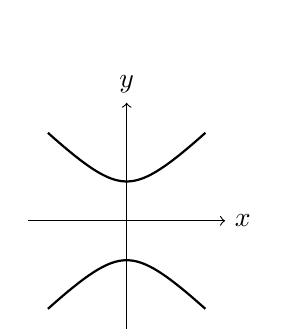
\begin{tikzpicture}[scale=0.5]
            \draw[->] (-2.5,0)--(2.5,0) node[right]{$x$};
            \draw[->] (0,-3)--(0,3) node[above]{$y$};
            \draw[thick,domain=-2:2,samples=50] plot (\x,{sqrt(\x*\x+1)});
            \draw[thick,domain=-2:2,samples=50] plot (\x,{-sqrt(\x*\x+1)});
        \end{tikzpicture}
    \end{choices}
\end{question}

\begin{solution}
    下列哪个图像表示 $x^2-y^2=1$？ \\
    标准式中 $a^2=b^2=1$，焦点在 $x$ 轴上，渐近线为 $y=\pm x$，图像为开口朝左右的双曲线。 \\
    故选 C。
\end{solution}
%endregion

%region 范围：圆锥曲线 | 考点：由焦点与短轴长求椭圆方程 | 难度：中等
\begin{question}
    已知椭圆的短轴长为 $12$，焦点是 $(-1,-2)$ 和 $(-1,7)$，求椭圆方程。 \paren[2]
    \begin{choices}
        \item $\dfrac{4\left(y-\frac52\right)^2}{225}+\dfrac{(x+1)^2}{36}=1$
        \item $\dfrac{4(x+1)^2}{225}+\dfrac{\left(y-\frac52\right)^2}{36}=1$
        \item $\dfrac{4y^2}{225}+\dfrac{(x+1)^2}{36}=1$
        \item $\dfrac{\left(y-\frac52\right)^2}{36}+\dfrac{4(x+1)^2}{225}=1$
    \end{choices}
\end{question}

\begin{solution}
    已知椭圆的短轴长为 $12$，焦点是 $(-1,-2)$ 和 $(-1,7)$，求椭圆方程。 \\
    中心为两焦点中点，$c$ 为中心到焦点的距离，短轴长 $2b=12$ 得 $b$，再由 $a^2=b^2+c^2$ 求 $a^2$。 \\
    \begin{align*}
        \text{中心} &= \left(-1,\frac52\right) \\
        c &= \frac92,\quad b=6
    \end{align*}
    \begin{align*}
        a^2 &= b^2+c^2 \\
        &= 36+\frac{81}{4} \\
        &= \frac{225}{4}
    \end{align*}
    \[
        \frac{4\left(y-\frac52\right)^2}{225}+\frac{(x+1)^2}{36}=1
    \]
    故选 A。
\end{solution}
%endregion

%region 范围：空间向量 | 考点：空间向量基本定理，用基底表示向量 | 难度：中等
\begin{question}
    如图，长方体 $OABCDEFG$ 中，$\overrightarrow{OA}=\underline{a}$，$\overrightarrow{OB}=\underline{b}$，$\overrightarrow{OC}=\underline{c}$，用 $\underline{a},\underline{b},\underline{c}$ 表示 $\overrightarrow{FA}$。
    \begin{center}
    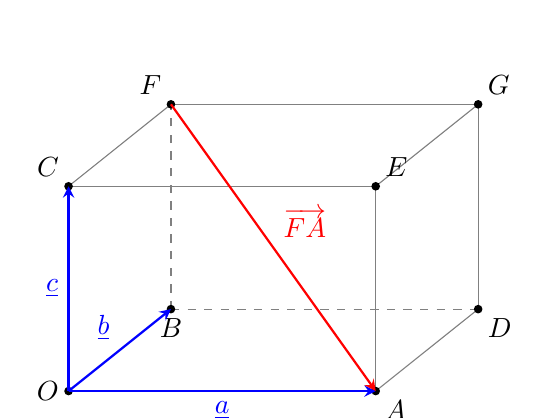
\begin{tikzpicture}[scale=1.3, >=stealth]
        \usetikzlibrary{calc}
        \coordinate (O) at (0,0);
        \coordinate (A) at (3,0);
        \coordinate (C) at (0,2);
        \coordinate (E) at (3,2);
        \coordinate (offset) at (1,0.8);
        \coordinate (B) at ($(O)+(offset)$);
        \coordinate (D) at ($(A)+(offset)$);
        \coordinate (F) at ($(C)+(offset)$);
        \coordinate (G) at ($(E)+(offset)$);

        \draw[gray, dashed] (O)--(B);
        \draw[gray, dashed] (B)--(D);
        \draw[gray, dashed] (B)--(F);
        \draw[gray] (O)--(A)--(E)--(C)--cycle;
        \draw[gray] (A)--(D);
        \draw[gray] (C)--(F);
        \draw[gray] (E)--(G);
        \draw[gray] (D)--(G)--(F);

        \foreach \p in {O,A,B,C,D,E,F,G}{\fill (\p) circle (1.2pt);}
        \node[left] at (O) {$O$};
        \node[below right] at (A) {$A$};
        \node[below] at (B) {$B$};
        \node[above left] at (C) {$C$};
        \node[below right] at (D) {$D$};
        \node[above right] at (E) {$E$};
        \node[above left] at (F) {$F$};
        \node[above right] at (G) {$G$};

        \draw[->, thick, blue] (O)--(A) node[midway, below] {$\underline{a}$};
        \draw[->, thick, blue] (O)--(B) node[midway, above left] {$\underline{b}$};
        \draw[->, thick, blue] (O)--(C) node[midway, left] {$\underline{c}$};
        \draw[->, thick, red] (F)--(A) node[midway, above right] {$\overrightarrow{FA}$};
    \end{tikzpicture}
    \end{center}
    \paren[2]
    \begin{choices}
        \item $\underline{a}-\underline{b}-\underline{c}$
        \item $\underline{b}+\underline{c}-\underline{a}$
        \item $\underline{a}+\underline{b}-\underline{c}$
        \item $\underline{a}-\underline{b}+\underline{c}$
    \end{choices}
\end{question}

\begin{solution}
    如图，长方体中 $\overrightarrow{OA}=\underline{a}$，$\overrightarrow{OB}=\underline{b}$，$\overrightarrow{OC}=\underline{c}$，用 $\underline{a},\underline{b},\underline{c}$ 表示 $\overrightarrow{FA}$。 \\
    $F$ 是 $B,C$ 两条棱方向张成的对角顶点，故 $\overrightarrow{OF}=\underline{b}+\underline{c}$，再用三角形法则求 $\overrightarrow{FA}$。 \\
    \begin{align*}
        \overrightarrow{OF} &= \underline{b}+\underline{c} \\
        \overrightarrow{FA} &= \overrightarrow{OA}-\overrightarrow{OF} \\
        &= \underline{a}-\underline{b}-\underline{c}
    \end{align*}
    故选 A。
\end{solution}
%endregion

%region 范围：空间向量 | 考点：线段外分点坐标公式 | 难度：中等
\begin{question}
    已知点 $A(16,8,-2)$ 及点 $B(7,2,1)$，求将线段 $AB$ 外分成 $5:2$ 的点 $C$ 的坐标。 \paren[2]
    \begin{choices}
        \item $(1,-2,3)$
        \item $(10,\frac{16}{3},0)$
        \item $(-8,-4,4)$
        \item $(22,14,-5)$
    \end{choices}
\end{question}

\begin{solution}
    已知点 $A(16,8,-2)$ 及点 $B(7,2,1)$，求将线段 $AB$ 外分成 $5:2$ 的点 $C$ 的坐标。 \\
    外分点公式：$C=\dfrac{mB-nA}{m-n}$，代入 $m=5,\ n=2$。 \\
    \begin{align*}
        C &= \frac{5B-2A}{5-2} \\
        &= \frac{5(7,2,1)-2(16,8,-2)}{3} \\
        &= \frac{(3,-6,9)}{3} \\
        &= (1,-2,3)
    \end{align*}
    故选 A。
\end{solution}
%endregion

%region 范围：平面向量 | 考点：由数量积求向量夹角 | 难度：基础
\begin{question}
    已知 $\underline{a}\cdot\underline{b}=-\dfrac12$，且 $\underline{a},\underline{b}$ 都是单位向量，求向量 $\underline{a}$ 与向量 $\underline{b}$ 的夹角。 \paren[2]
    \begin{choices}
        \item $60^\circ$
        \item $120^\circ$
        \item $150^\circ$
        \item $30^\circ$
    \end{choices}
\end{question}

\begin{solution}
    已知 $\underline{a}\cdot\underline{b}=-\dfrac12$，且 $\underline{a},\underline{b}$ 都是单位向量，求向量 $\underline{a}$ 与向量 $\underline{b}$ 的夹角。 \\
    单位向量满足 $|\underline{a}|=|\underline{b}|=1$，代入 $\cos\theta=\dfrac{\underline{a}\cdot\underline{b}}{|\underline{a}||\underline{b}|}$。 \\
    \begin{align*}
        \cos\theta &= \frac{-\frac12}{1\times1} \\
        &= -\frac12
    \end{align*}
    \[
        \theta = 120^\circ
    \]
    故选 B。
\end{solution}
%endregion
%region 范围：平面向量 | 考点：由模长关系求数量积 | 难度：基础
\begin{question}
    已知 $|\underline a|=3$，$|\underline b|=8$，$|\underline a-\underline b|=2\sqrt{14}$，求 $\underline a\cdot\underline b$。 \paren[2]
    \begin{choices}
        \item $\dfrac{17}{2}$
        \item $17$
        \item $-\dfrac{17}{2}$
        \item $28$
    \end{choices}
\end{question}

\begin{solution}
    已知 $|\underline a|=3$，$|\underline b|=8$，$|\underline a-\underline b|=2\sqrt{14}$，求 $\underline a\cdot\underline b$。 \\
    利用 $|\underline a-\underline b|^2=|\underline a|^2-2\underline a\cdot\underline b+|\underline b|^2$ 展开求解。 \\
    \begin{align*}
        (2\sqrt{14})^2 &= 3^2-2\underline a\cdot\underline b+8^2 \\
        56 &= 73-2\underline a\cdot\underline b \\
        2\underline a\cdot\underline b &= 17
    \end{align*}
    \[
        \underline a\cdot\underline b = \frac{17}{2}
    \]
    故选 A。
\end{solution}
%endregion

%region 范围：空间向量 | 考点：向量叉积（外积）的计算与平行向量的判断 | 难度：中等
\begin{question}
    已知向量 $\underline a=-2i+j+2k$ 与 $\underline b=4i-2j-4k$，求外积 $\underline a\times\underline b$。 \paren[2]
    \begin{choices}
        \item $\underline 0$
        \item $8i+8j+8k$
        \item $-8i-8j-8k$
        \item $16i+16j+16k$
    \end{choices}
\end{question}

\begin{solution}
    已知向量 $\underline a=-2i+j+2k$ 与 $\underline b=4i-2j-4k$，求外积 $\underline a\times\underline b$。 \\
    按行列式展开计算叉积各分量。 \\
    \begin{align*}
        \underline a\times\underline b &=
        \begin{vmatrix}
            i & j & k \\
            -2 & 1 & 2 \\
            4 & -2 & -4
        \end{vmatrix} \\
        &= i(1\times(-4)-2\times(-2)) - j((-2)\times(-4)-2\times4) + k((-2)\times(-2)-1\times4)
    \end{align*}
    \[
        \underline a\times\underline b = 0i+0j+0k = \underline 0
    \]
    故选 A。
\end{solution}
%endregion

\vfill % 与上方内容保持距离

\noindent
\newlength{\sigwidth}
\settowidth{\sigwidth}{（\hspace{4em}师）}

\begin{tabular*}{\textwidth}{@{\extracolsep{\fill}} l l l}
    出题： & 审题： & 审核： \\[4em]
    \rule{\sigwidth}{0.5pt} &
    \rule{\sigwidth}{0.5pt} &
    \rule{\sigwidth}{0.5pt} \\
    （\hspace{0em} \setterteacher ） &
    （\hspace{0em} \reviewteacher ）  &
    （\hspace{0em} \auditteacher ） \\
\end{tabular*}

\clearpage
\thispagestyle{empty} % 取消这一页的页眉页脚（页码）
~
\clearpage
\end{document}
